
\chapter{Examples}
\label{chap:Examples}

In this chapter we describe 4 examples: 1) a closed-set
identification task, 2) an adaptive speech in noise identification
task, and 3) an adaptive just noticeable difference task (gap
detection), and 4) same as 3, but modified to the attention span
and interest of young children. Each example consists of 1) a
general description, 2) the concept, and 3) the implementation in
XML.

It is advised to run the experiment before reading the details.
The experiment files are stored in the \apex directory under
\filename{examples/manual} in the \apex folder, together with
sound files and figures of the respective experiments. Note again:
if the experiment file has the extension ``.apx'' it remains an
XML file that can be edited with OxygenXML. The results file will
automatically have the extension ``.results''. \textbf{(needs to
be done)}.


\newpage
\section{Example 1: Closed-set identification of words in noise with
figures}

\subsection{General description of the experiment} See
\filename{examples/manual/closedsetword.apx}. This is an example
of a closed-set identification test for children. A word (wave
file) is presented and the child responds by clicking on one of
four figures on the screen(figure~\ref{fig:closedset}).
Subsequently, a new set of figures is shown, and again, a word
corresponding to one of these figures is routed to the sound card.
This is repeated 3 times. The three words are embedded in noise at
a certain signal-to-noise ratio. In this example the level of the
noise is fixed and the level of the word varies. At the beginning
of the experiment \apex queries for the SNR (signal to noise
ratio, in dB). After having entered this value four figures will
appear. Press Start to start the experiment and to hear the first
stimulus (speech in noise). After the experiment has finished the
results are written to a results file and the percentage correct
is determined.

\index{Example: closed-set identification}

\begin{figure}
 \centering
%% 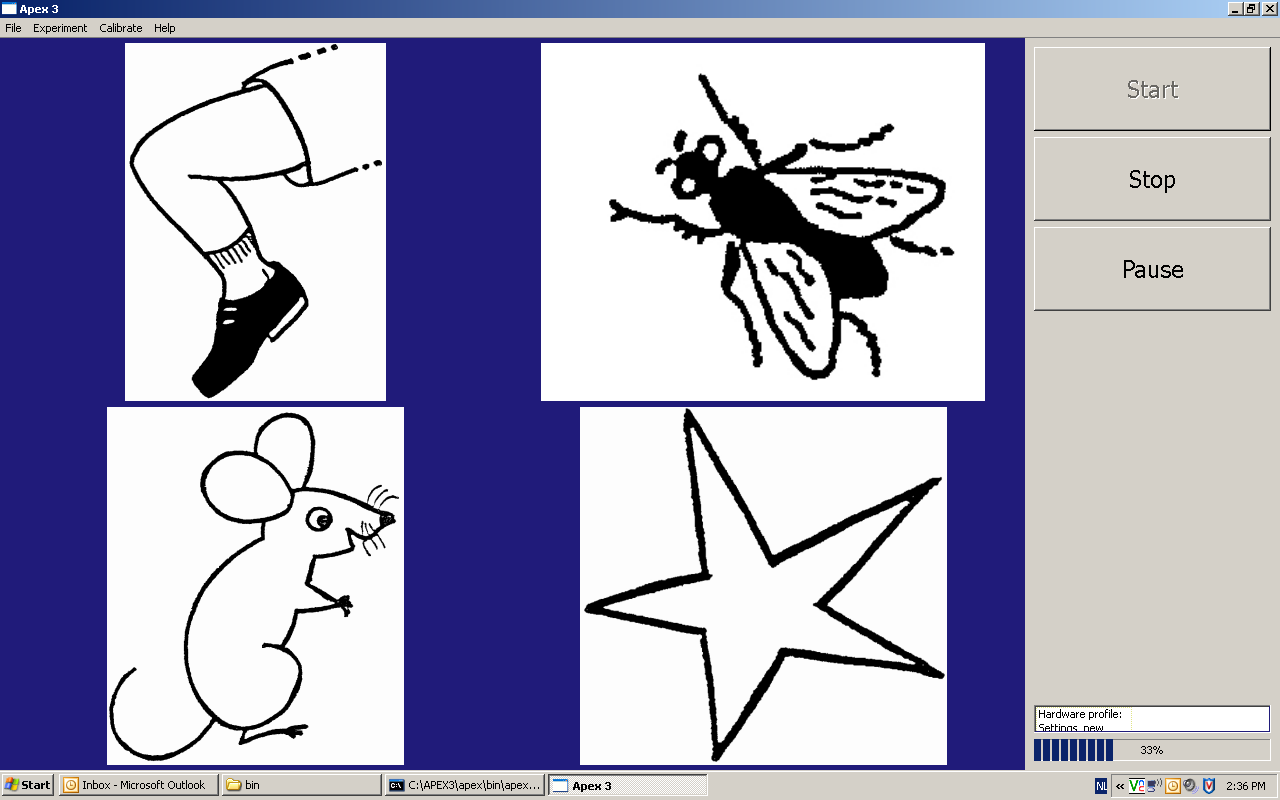
\includegraphics[width=\textwidth]{example1closedset.png}
 \caption{Example of closed-set identification experiment}
 \label{fig:closedset}
\end{figure}

\subsection{Conceptual}
The experiment as described in the previous paragraph should first
be translated to concepts understood by \apex. The main concepts
in this example are \textbf{datablock}, \textbf{stimulus},
\textbf{screen} and \textbf{procedure}. For each of the 3 words to
be presented to the subject, a wave file is available on disk. For
each wave file, a datablock is defined, and for each resulting
datablock a stimulus is defined. Everything that is defined is
assigned an ID, to be able to refer to it later on. Therefore, now
we have 3 stimuli with IDs \id{stimulus_star}, \id{stimulus_mouse}
and \id{stimulus_fly}.

We should also define the things to be shown on the screen during
the experiment. This is done by defining a screen for each word.
Each screen contains 4 pictures, of which one corresponds to the
word. Each screen again gets an ID, in this case we name the
screen by the pictures it contains. Therefore we now have 3
screens with ID \id{screenstar_horse_vase_moon},
\id{screenknee_fly_mouse_star} and \id{screenmouse_fly_star_moon}.

To indicate the order in which the words should be presented, and
together with which screen, a procedure is defined. In the
procedure a number of trials is defined. Recall that a trial is
the combination of a screen, a stimulus and a correct answer.
Therefore a trial is a way to link each of our stimuli with a
screen.

Now only the output logic remains to be defined. The idea is to
continuously present a noise signal and to set the level of the
words such that a certain SNR is obtained. To achieve this, we
define 2 filters, the first one is a generator (i.e., a filter
without input channels) that will generate the noise signal. The
other one is an amplifier, which will amplify or attenuate the
words to obtain the desired SNR.

In the following sections each of the elements of the \xml{XML}
file necessary to implement the latter concepts will be described
in detail. The first one is \element {procedure}.

\subsection{Detailed description of various elements}
\begin{lstlisting}
  <procedure xsi:type="apex:constantProcedureType">
    <parameters>
      <presentations>1</presentations>
      <order>sequential</order>
    </parameters>
    <trials>
      <trial id="trial_star">
        <answer>picturestar</answer>
        <screen id="screenstar_horse_vase_moon"/>
        <stimulus id="stimulus_star"/>
      </trial>
      <trial id="trial_fly">
        <answer>picturefly</answer>
        <screen id="screenknee_fly_mouse_star"/>
        <stimulus id="stimulus_fly"/>
      </trial>
      <trial id="trial_mouse">
        <answer>picturemouse</answer>
        <screen id="screenmouse_fly_star_moon"/>
        <stimulus id="stimulus_mouse"/>
      </trial>
    </trials>
  </procedure>
\end{lstlisting}

The attribute \xml{xsi:type="apex:constantProcedureType"}
indicates that a constant stimuli procedure is used. This means
that the procedure will select the next trial from the trial list
and that it completes after every trial has been presented a
certain number of times.
\begin{itemize}

\item \element{parameters} defines the behavior of the procedure
\begin{itemize}

\item \element{presentations} every trial is presented once

\item \element{order} \xml{sequential} the three trials are
presented sequentially, in the order that is specified in the
experiment file
\end{itemize}
\index{presentations} \index{order}

\item \element{trials} contains different \element{trial} elements
to specify a trial. After selecting a trial the
\element{procedure} will show the specified screen and send the
stimulus to the device. Each trial is given an ID (arbitrary
name), eg \id{TrialStar}, such that it can be referred to later on
or viewed in the results file.

\item \element{answer} the correct answer, to be used by \apex to
determine whether the subject's response is correct. Here, the
subject gets the opportunity to click on one of 4 pictures. The
result from the screen (the subject's response) will be the ID of
the element of the screen that was clicked. Therefore, in this
example, we specify the ID of the picture corresponding to the
stimulus that is presented.
\end{itemize}

A trial must be defined for all the words of the experiment.

\index{trial} \index{answer} \index{screen} \index{stimulus}

\begin{lstlisting}
    <corrector xsi:type="apex:isequal"/>
\end{lstlisting}
\index{corrector}

The corrector checks whether the response is correct or not. The
attribute \xml{xsi:type="apex:isequal"} compares whether the two
input values are exactly the same. In this example
\element{corrector} compares the answer specified under trial and
the ID corresponding to the picture that has been clicked.

\begin{lstlisting}
<screens>
    <uri_prefix>closedset</uri_prefix>
    <reinforcement>
      <progressbar>true</progressbar>
      <feedback length="600">false</feedback>
    </reinforcement>
    <screen id="screenstar_horse_vase_moon">
      <gridLayout height="2" width="2">
        <picture id="picturestar" row="1" col="1">
          <path>star.jpg</path>
        </picture>
        <picture id="picturehorse" row="2" col="1">
          <path>horse.jpg</path>
        </picture>
        <picture id="picturevase" row="1" col="2">
          <path>vase.jpg</path>
        </picture>
        <picture id="picturemoon" row="2" col="2">
          <path>moon.jpg</path>
        </picture>
            </gridLayout>
      <buttongroup id="buttongroup1">
        <button id="picturestar"/>
        <button id="picturehorse"/>
        <button id="picturevase"/>
        <button id="picturemoon"/>
                </buttongroup>
      <default_answer_element>buttongroup1</default_answer_element>
    </screen>
    <screen id="screenknee_fly_mouse_star">
      <gridLayout height="2" width="2">
        <picture id="pictureknee" row="1" col="1">
          <path>knee.jpg</path>
        </picture>
        <picture id="picturefly" row="2" col="1">
          <path>fly.jpg</path>
        </picture>
        <picture id="picturemouse" row="1" col="2">
          <path>mouse.jpg</path>
        </picture>
        <picture id="picturestar" row="2" col="2">
          <path>star.jpg</path>
        </picture>
      </gridLayout>
      <buttongroup id="buttongroup2">
        <button id="pictureknee"/>
        <button id="picturefly"/>
        <button id="picturemouse"/>
        <button id="picturestar"/>
      </buttongroup>
      <default_answer_element>buttongroup2</default_answer_element>
    </screen>
    <screen id="screenmouse_fly_star_moon">
      <gridLayout height="2" width="2">
        <picture id="picturemouse" row="1" col="1">
          <path>mouse.jpg</path>
        </picture>
        <picture id="picturefly" row="2" col="1">
          <path>fly.jpg</path>
        </picture>
        <picture id="picturestar" row="1" col="2">
          <path>star.jpg</path>
        </picture>
        <picture id="picturemoon" row="2" col="2">
          <path>moon.jpg</path>
        </picture>
      </gridLayout>
      <buttongroup id="buttongroup3">
        <button id="picturemouse"/>
        <button id="picturefly"/>
        <button id="picturestar"/>
        <button id="picturemoon"/>
      </buttongroup>
      <default_answer_element>buttongroup3</default_answer_element>
    </screen>
  </screens>
\end{lstlisting}

\element{screens} contains several \element{screen} elements that
can be referred to elsewhere in the experiment file (e.g., in
\element{procedure} above).

\begin{itemize}
\item \element{uri_prefix} a relative path is specified here
(relative with respect to the experiment file). Since \apex knows
the location of the experiment file, only the folder containing
the wave files and pictures must be specified. It is also possible
to give the absolute path, starting at the root. There are 3 ways
to specify a prefix: by directly specifying an absolute path, by
directly specifying a path relative to the experiment file or by
referring to a prefix stored in \filename{apexconfig.xml}. Please
refer to section~\ref{sec:prefixes} for more information.

\item \element{reinforcement} includes

\begin{itemize}

\item \element{progressbar} As the value is \xml{true} a
progressbar will be displayed in the right hand bottom corner of
the screen that indicates how many trials have been completed and
how many remain.

\item \element{feedback length} duration of time after response
(in msec) that \apex waits before presenting the next trial.
During this interval, feedback can be displayed. In this case, no
feedback (thumb up, thumb down) is given as the value is
\xml{false}.

\end{itemize}
\end{itemize}

\begin{itemize}
\item \element{screen} For each word to be presented, a screen is
defined. Each screen has an ID by which it can be referred to
elsewhere in the experiment file (e.g. in \element{trials} to
associate it with a stimulus).
\begin{itemize}

\item \element{gridLayout} specifies how the four figures will be
arranged on the screen. A GridLayout creates a regular grid on the
screen with the specified number of rows and columns. In this
example there are 2 rows and 2 columns. Each figure is defined by
means of a \element{picture} element. Such a definition can be
seen as associating a graphics file with an ID and specifying at
what position of the layout it should be shown. In this case, jpeg
files are used, but other formats are also possible (e.g., png,
bmp, gif).

\begin{itemize}
\item \element{picture}


\element{uri} since the prefix as specified under
\element{uri_prefix} is preprended to each \element {uri}  it
suffices to give the name of the .jpeg file in \element{path}. The
path is relative to the experiment file.

\end{itemize}
\end{itemize}
\begin{itemize}
\item \element{buttongroup} defines a group of screen elements,
namely those (four figures) that are displayed on the screen. The
ID is defined before.

\item \element{default_answer_element} As many elements can be
defined in a screen, \apex has no way to know which element
contains the subject's response. If, for example, a text box is
shown and 2 buttons, it is unclear which is to be used to
determine whether the answer is correct or not. Therefore, in
\element{default_answer_element} the element is designated that
contains the subject's response. In the case of screen elements
that are clicked in order to respond, the example is further
complicated by the fact that we cannot specify just one of the
elements (buttons, pictures), but the response rather comes from a
group of elements. This is when a \element{buttongroup} can be
used to group together different screen elements.
\end{itemize}
\end{itemize}
\index{screens} \index{uri prefix} \index{reinforcement}
\index{progressbar} \index{feedback length} \index{screen}
\index{gridlayout} \index{picture} \index{path}
\index{buttongroup} \index{default answer element}

In this example 5 datablocks are defined, 3 for the word files, 1
for the noise and 1 for silence.

\begin{lstlisting}
 <datablocks>
    <uri_prefix>closedset/</uri_prefix>
    <datablock id="datablock_star">
      <device>wavdevice</device>
      <uri>star.wav</uri>
    </datablock>
    <datablock id="datablock_fly">
      <device>wavdevice</device>
      <uri>fly.wav</uri>
    </datablock>
    <datablock id="datablock_mouse">
      <device>wavdevice</device>
      <uri>mouse.wav</uri>
    </datablock>
    <datablock id="noisedata">
      <device>wavdevice</device>
      <uri>noise.wav</uri>
    </datablock>
    <datablock id="silence">
      <device>wavdevice</device>
      <uri>silence:500</uri>
    </datablock>
  </datablocks>
\end{lstlisting}
\index{datablocks}

\element{datablocks} contains 5 \element{datablock} elements and a
prefix.
\begin{itemize}
\item \element{uri_prefix} a relative path is specified here. It
is also possible to give the absolute path, starting at the root
(see section~\ref{sec:prefixes}).

\item \element{datablock} For each wave file a datablock is made,
with an ID.  \item Each datablock is associated to a
\element{device} (by means of the ID of the device). In datablock
\id{silence} the special syntax is demonstrated for creating a
datablock containing only silence (i.e., all samples are zeros).
This is done to prevent the speech and noise from starting at the
same time. The length of the silence datablock is specified in ms
after the prefix \xml{silence}. It is added before the signal, not
before the noise.

\end{itemize}
\index{datablocks} \index{uri prefix} \index{datablock}
\index{device} \index{uri}

A datablock must be made for all wave files used in the
experiment, including the noise (that will be used by the noise
generator).



In the next sections, the output logic will be defined.
Figure~\ref{fig:ex1-output} gives an overview of the building
blocks that are used in this example. On the left hand side the
datablocks are shown. In the middle the noise generator and the
amplifier and on the right hand side the sound card. As the words
are to be amplified or attenuated according to the desired SNR,
the corresponding datablocks are routed through the amplifier.

\begin{figure}
 \centering
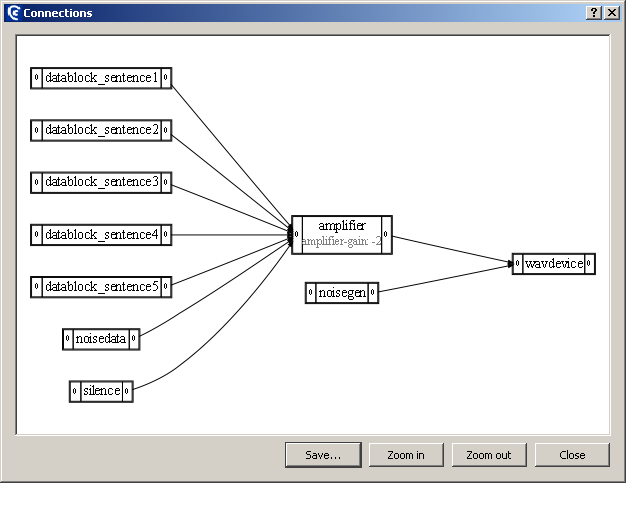
\includegraphics[width=0.5\textwidth]{connectionswindow.png}
 \caption{The connection window}
 \label{fig:ex1-output}
\end{figure}

In the next element the output device is specified.

\begin{lstlisting}
 <devices>
    <device id="wavdevice" xsi:type="apex:wavDeviceType">
      <driver>portaudio</driver>
      <card>default</card>
      <channels>1</channels>
      <samplerate>44100</samplerate>
    </device>
  </devices>

\end{lstlisting}
\index{devices}

All devices defined in the experiment file are grouped in
\element{devices}. In this example there is only 1
\element{device} element. Its ID is set to \id{soundcard}. As an
ID is unique for an entire experiment file, it can be used later
on to refer to this device.

\begin{itemize}
\item  The \xml{xsi:type="apex:wavDeviceType"} attribute tells
\apex that a sound card is used. The experiment only starts if all
devices can be opened.

\item \element{driver} specifies the software driver to be used
for sound output. If unsure, set it to \xml{portaudio}.

\item \element{card} specifies the name of the sound card to be
used. The system default card can be used by specifying
\xml{default} as a card name. Other card names can be defined in
\filename{apexconfig}.

\item \element{channels} specifies the number of channels of the
sound card to be used. The number of channels is restricted to the
selected sound card, with a maximum of 2 for portaudio.

\item \element{samplerate} the sampling rate of the sound card;
Not all sampling rates are supported by all devices, and some
drivers automatically convert the sampling rate. Check your sound
card documentation. The sample rate of the sound card should
correspond to the sampling rates of all datablocks used with it.
If not, an error message will be shown.

\end{itemize}

\index{device} \index{driver} \index{card} \index{channels}
\index{gain} \index{samplerate}

Filters must be defined whenever the signal (or noise) is
manipulated. In this example the level of the noise remains
constant and the signal is amplified or attenuated using an
amplifier filter (loop of \element{datablock}).

\begin{lstlisting}
<filters>
    <filter xsi:type="apex:dataloop" id="noisegen"> (*@\label{xml:filter1}@*)
      <device>wavdevice</device>
      <channels>1</channels>
      <continuous>false</continuous>
      <datablock>noisedata</datablock>
      <basegain>-5</basegain>
      <gain id="noisegain">0</gain>
      <randomjump>true</randomjump>
    </filter>
    <filter xsi:type="apex:amplifier" id="amplifier">  (*@\label{xml:filter2}@*)
      <device>wavdevice</device>
      <channels>1</channels>
      <basegain>-5</basegain>
      <gain id="gain">0</gain>
    </filter>
  </filters>
\end{lstlisting}
\index{filter}

\element{filters} contains individual \element{filter} elements,
which specify a filter, or as a special case a generator (i.e., a
filter without input channels).
\begin{itemize}

\item \element{filter} on line~\ref{xml:filter1} the attribute
\xml{xsi:type="apex:dataloop"} tells \apex that a dataloop
generator has to be created. This is a generator that takes a
datablock and loops it infinitely. The datablock to be looped is
specified by its ID \id{noisedata}. The dataloop generator itself
is assigned the ID \id{noisegen}.


\item \element{filter} on line~\ref{xml:filter2} the attribute
\xml{xsi:type="apex:amplifier"} tells \apex that an amplifier is
to be created. The gain of this amplifier will be varied to change
the amplitude of the words and thus the SNR. It is assigned ID
\id{amplifier}. The gain of the amplifier is made a variable
parameter by assigning it ID \id{gain}
\begin{itemize}
\item \element{device} The device with which the filter is
associated \item \element{channels} The number of channels of the
filter. The available number of channels is dependent on the type
of filter. An amplifier can have any number of channels.

\item If \element{continuous} is set to \xml{true}, the filter or generator
will keep on running in between two trials (i.e., when the subject is responding).
 In this example it stops when the stimulus stops playing (\xml{false}).

\item \element{datablock} The datablock with ID noisedata,
specified under \element{datablocks} will be looped.

\item \element{basegain} the total gain of the amplifier is
basegain+gain. Basegain cannot be a parameter, gain can be a
parameter. The total gain of the complete output system should not
be larger than 0 to avoid clipping of the signal. This is why
basegain = -5.

\item \element{gain} extent to which the signal is amplified.

\item If \element{randomjump} is set to \xml{true}, when the dataloop is started, it will jump to a random sample in the datablock. Thereafter it is looped.
\end{itemize}
\end{itemize}

\index{filters} \index{filter} \index{device} \index{channels}
\index{continuous} \index{datablock} \index{basegain} \index{gain}
\index{randomjump}

\begin{lstlisting}
<stimuli>
    <stimulus id="stimulus_star">
      <datablocks>
        <sequential>
          <datablock id="silence"/>
          <datablock id="datablock_star"/>
          <datablock id="silence"/>
        </sequential>
      </datablocks>
    </stimulus>
    <stimulus id="stimulus_fly">
      <datablocks>
        <sequential>
          <datablock id="silence"/>
          <datablock id="datablock_fly"/>
          <datablock id="silence"/>
        </sequential>
      </datablocks>
    </stimulus>
    <stimulus id="stimulus_mouse">
      <datablocks>
        <sequential>
          <datablock id="silence"/>
          <datablock id="datablock_mouse"/>
          <datablock id="silence"/>
        </sequential>
      </datablocks>
    </stimulus>
  </stimuli>
\end{lstlisting}
\index{stimuli} \index{datablocks}


\element{stimuli} contains different \element{stimulus}, each with
an ID \element{stimulus}

\begin{itemize}\item \element{datablocks}
can be combined in \element{sequential} order (as opposed to
\element{simultaneous}.
\end{itemize}

This is repeated for all the stimuli in the experiment.

\index{stimuli} \index{stimulus} \index{datablocks}
\index{sequential}

\begin{lstlisting}
<connections>
    <connection>
      <from>
        <id>_ALL_</id>
        <channel>0</channel>
      </from>
      <to>
        <id>amplifier</id>
        <channel>0</channel>
      </to>
    </connection>
    <connection>                (*@\label{xml:cha}@*)
      <from>
        <id>amplifier</id>
        <channel>0</channel>
      </from>
      <to>
        <id>wavdevice</id>
        <channel>0</channel>
      </to>
    </connection>               (*@\label{xml:chb}@*)
    <connection>                (*@\label{xml:chc}@*)
      <from>
        <id>noisegen</id>
        <channel>0</channel>
      </from>
      <to>
        <id>wavdevice</id>
        <channel>0</channel>
      </to>
    </connection>               (*@\label{xml:chd}@*)
  </connections>

\end{lstlisting}
\index{connections}

\index{channel}

\element{connections} defines how the different datablocks and
filters are routed to the output device. The ID \id{_ALL_} stands
for all the datablocks. In this example they are routed to the
first channel of the filter with ID {amplifier} (defined under
\element{filters}). In the amplifier the signal is amplified or
attenuated and sent to the wavdevice on lines~\ref{xml:cha}
to~\ref{xml:chb}. At the same time the noise, generated by a
generator with ID noisegen, is sent to the same channel of the
wavdevice. The channels are numbered from 0 onwards. The level of
the noise remains constant and does not pass through an amplifier
(lines~\ref{xml:chc} to~\ref{xml:chd}).

A visual representation of connections can be obtained by choosing
``Show stimulus connections'' under ``Experiment''in the main
\apex menu (top left menu bar).



\begin{lstlisting}
<results>
   <xsltscript>idn.xsl</xsltscript>
</results>
\end{lstlisting}

Even if \element{results} is not specified in the experiment file
\apex will deliver a results file in XML.
\begin{itemize}
\item \element{xsltscript}  a script can transform the XML data to
an easier readable format; this script can be stored in folder
\filename{scripts} under \apex. For more information please read
section~\ref{sec:Using XSLT transforms}.
\end{itemize}
\index{results} \index{xsltscript}

\begin{lstlisting}
<interactive>
   <entry type="int" description="SNR in dB"
    expression="/apex:apex/filters/filter[@id='amplifier']/gain"
    default="0"/>
 </interactive>
\end{lstlisting}

If a small part of an experiment file has to be changed right
before the start of an experiment (e.g. a start value, a gain
value, the subject's name), \apex can show the experimenter a
small \ac{gui} containing the elements to be changed. This is
accomplished by defining the \element{interactive} element in the
experiment file.

In this example we will modify the gain of the filter with ID
\id{amplifier} to a value that is entered by the experimenter at
the start of the experiment.

It is only possible to change the value of an existing element of the experiment file, elements cannot be added. For each element to be changed, an \element{entry} should be defined under \element{interactive}. \element{entry} has  four attributes that should be defined:

\begin{itemize}
\item \attribute{type} specifies the type of input element that
will be shown. If it is \xml{int}, a spinbox\footnote{A spinbox is
an input field that only accepts numbers and has 2 buttons to
respectively increase or decrease its value} will be shown. If it
is \xml{string} a plain text box will be shown. In this case a
spinbox will be shown as a gain is always numeric. \item
\attribute{description} defines the text to be shown in the
\ac{gui} next to the input element, such that the experimenter
knows exactly what to fill in. \item \attribute{expression}
defines the element of the experiment file to be changed. It is
specified by a so-called XPath expression \footnote{see
\url{http://www.w3.org/TR/xpath}}. For a description of XPath, we
refer to the according standard or a good XML book.

\oxygen{OxygenXML can generate XPath expressions for you. First
point the cursor to the target element, then click the right mouse
button and select. An XPath expression to the clicked location is
now in the clipboard and can be pasted at the appropriate place
using the paste function.} \item \attribute{default} specifies the
default value to be shown in the input element.
\end{itemize}

\index{interactive} \index{entry type} \index{expression}

\begin{lstlisting}
<general>
    <showresults>true</showresults>
    <saveprocessedresults>true</saveprocessedresults>
</general>
\end{lstlisting}

\element{general} defines some general parameters. Saving
processed results in a results file is only possible if a
XSLT-script is defined. See section~\ref{sec:Using XSLT
transforms}.

\begin{itemize}
\item \element{showresults} If \xml {true} a window will appear
after completion of the experiment asking whether the results
should be shown on screen.

\item \element{saveprocessedresults} If \xml {true} the
experimenter will be asked whether the processed results must be
appended to the results file.
\end{itemize}

\index{general} \index{showresults} \index{saveprocessedresults}

\newpage
\section{Example 2: Identification of speech in noise using an adaptive method}

\subsection{General description of the experiment}
See \filename{examples/manual/sentenceinnoise.apx}. This is an
example of an adaptive speech in noise test. It determines the
 \ac{srt}, the 50 percent correct point, using
the 1-down, 1-up method described by \citet{PM79}. In this
adaptive procedure the first sentence is repeated with increasing
level until it is identified correctly. Subsequently, the SRT is
determined by increasing or decreasing the level in steps of 2 dB,
according to the last response. Other decision procedures (eg
2-down 1-up) can also be implemented using \apex. In this example
the 5 sentences are scored on the basis of their keywords. The
keywords are indicated in bold on the screen. The
experimenter/clinician is seated in front of the screen and
decides whether the subject has repeated the keywords (of the
sentence) correctly, after which the correct or incorrect button
is clicked(figure~\ref{fig:sentencenoise}). No feedback is
provided. The starting level is given in signal-to noise ratio
(the level of the noise remains the same, that of the signal
varies). In this example speech and noise are routed to the same
channel, i.e. one speaker or one earpiece of the headphone. The
results are written to a results file.

\begin{figure}
 \centering
 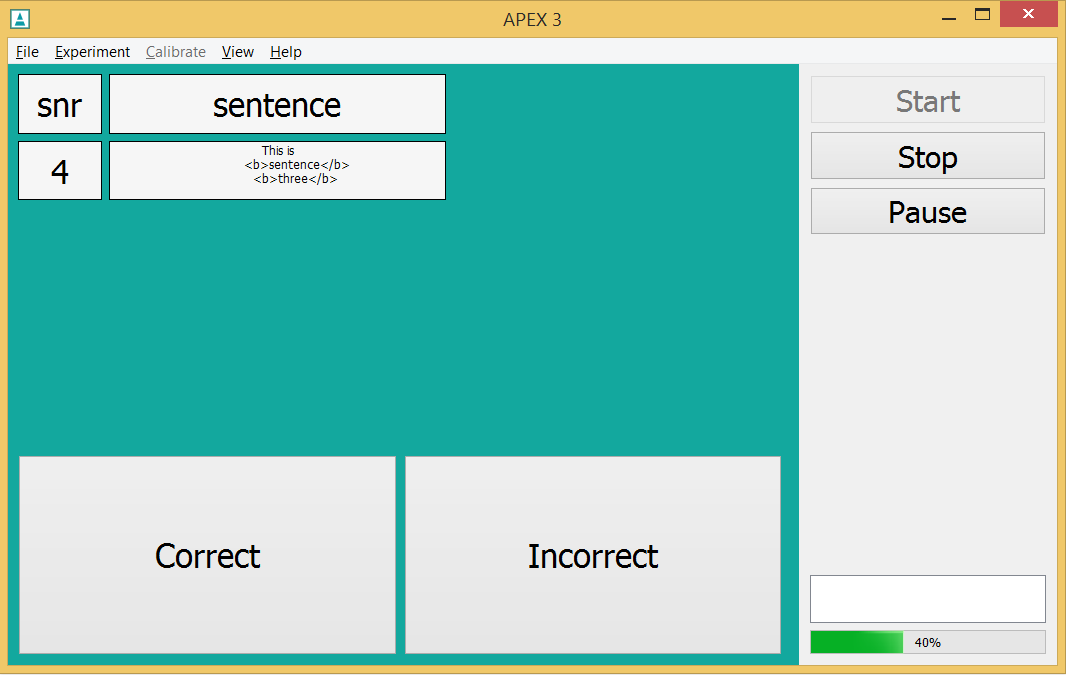
\includegraphics[width=\textwidth]{example2sentenceinnoise.png}
 \caption{Example of adaptive sentence in noise experiment}
 \label{fig:sentencenoise} \todo{bold werkt niet correct?}

\end{figure}
\subsection{Conceptual}
The experiment as described in the previous paragraph should first
be translated to concepts understood by \apex. The main concepts
in this example are \textbf{datablock}, \textbf{stimulus},
\textbf{screen}, \textbf{procedure}, a \textbf{variable} parameter
(to change the gain) and \textbf{fixed Parameter} to show a
sentence on the screen. For each sentence a datablock is defined,
and for each resulting datablock a stimulus is defined. As always,
everything that is defined, is assigned an ID, to be able to refer
to it later on. In this example there are 5 stimuli with IDs
\id{stimulus_sentence1}, \id{stimulus_sentence2},
\id{stimulus_sentence3}, \id{stimulus_sentence4} and
\id{stimulus_sentence5}. The procedure defines a number of trials.
Recall that a trial is the combination of a screen (always the
same in this example), a stimulus and a response.

As we are dealing with an adaptive procedure a fixed or variable
parameter is adapted. In this example a variable parameter is
adapted to change the gain of the sentence, and a fixed parameter
is used to show a sentence on the screen. The screen also shows
the signal-to-noise ratio (SNR) under test and the response
alternatives ``correct'' and ``incorrect''.

Now only the output logic remains to be defined. The idea is to
continuously present a noise signal and to vary the level of the
sentences adaptively. To achieve this, we define 2 filters, the
first one is a generator (i.e., a filter without input channels)
that will generate the noise signal. The other one is an
amplifier, which will amplify or attenuate the sentences to obtain
the desired SNR. Both are connected to one channel of the
wavdevice.

In the following sections each of the elements of the XML file
necessary to implement the latter concepts will be described in
detail.

\subsection{Detailed description of various elements}

\begin{lstlisting}
<procedure xsi:type="apex:adaptiveProcedure">
  <parameters>
    <presentations>1</presentations>
    <order>sequential</order>
    <corrector xsi:type="apex:isequal"/>
    <nUp>1</nUp>
    <nDown>1</nDown>
    <adapt_parameter>gain</adapt_parameter>
    <start_value>0</start_value>
    <stop_after_type>presentations</stop_after_type>
    <stop_after>1</stop_after>
    <larger_is_easier>true</larger_is_easier>
    <repeat_first_until_correct>true</repeat_first_until_correct>
    <stepsizes><stepsize begin="0" size="2"/></stepsizes>
  </parameters>

  <trials>
    <trial id="trial_sentence1">
         <answer>button_correct</answer>
         <screen id="screen"/>
         <stimulus id="stimulus_sentence1"/>
    </trial>

    <trial id="trial_sentence2">
         <answer>button_correct</answer>
         <screen id="screen"/>
         <stimulus id="stimulus_sentence2"/>
    </trial>

    <trial id="trial_sentence3">
        <answer>button_correct</answer>
        <screen id="screen"/>
        <stimulus id="stimulus_sentence3"/>
    </trial>

    <trial id="trial_sentence4">
        <answer>button_correct</answer>
        <screen id="screen"/>
        <stimulus id="stimulus_sentence4"/>
    </trial>

    <trial id="trial_sentence5">
        <answer>button_correct</answer>
        <screen id="screen"/>
        <stimulus id="stimulus_sentence5"/>
    </trial>
  </trials>
</procedure>
\end{lstlisting}


The attribute \xml{xsi:type="adaptiveProcedureType"} of
\element{procedure} refers to a procedure in which a parameter is
changed according to the response of the subject. In this example
the gain of the amplifier is adapted. The procedure selects the
next trial from the trial list and it completes after every trial
has been presented a certain number of times.

\begin{itemize}
\item \element{parameters} defines the behavior of the procedure

\begin{itemize}

\item \element{presentations} every trial is presented once

\item \element{order} the trials are presented sequentially, in
the order that is specified in the experiment file (if
\xml{random} would be specified, they would be presented in random
order).

\item \element{corrector} the corrector checks whether the response is correct or not. The
attribute \xml{xsi:type="apex:isequal"} compares whether the two
input values are exactly the same. In this example
\element{corrector} compares the answer specified under trial  (\id{button_correct}) and
the ID corresponding to the picture that has been clicked (either \id{button_correct} or \id{button_incorrect}).

\item \element{nUp} the level is increased after n (here 1)
incorrect response(s); cf \element{larger_is_easier}

\item \element{nDown} the level is decreased after n (here 1)
correct response(s); cf \element{larger_is_easier}

\item \element{adapt_parameter} to be adapted

\item \element{start_value} the experiment starts with gain=0
(input of user). The value here will be replaced by the entry
value. Please refer to section~\ref{sec:Interactive} for more
information.

\item \element{stop_after_type} the experiment stops after a
specified number of presentations of each trial is completed (it
is also possible to stop after \element{reversals}.

\item \element{stop_after} the experiment stops after 1
presentation of each trial

\item \element{larger_is_easier} If \xml{true}, then larger values
of the parameter are easier than smaller values. It is used to
determine \element{nUp} and \element{nDown}.

\item \element{repeat_first_until_correct} the first trial is
repeated with increasing gain until it is identified correctly.

\item \element{stepsizes} from the beginning of the experiment
(begin=0) the stepsize is 2 dB.
\end{itemize}

\item \element{trials} contains different \element{trial} elements
to specify a trial. Once a trial is selected, \element{procedure}
will show the specified screen and send the stimulus to the
device. Each trial is given an ID (arbitrary name), eg
\id{trialsentence1}, such that it can be referred to later on or
viewed in the results file. A trial must be defined for all the
sentences of the experiment.

\item \element{answer} the correct answer, to be used by \apex to
determine whether the subject's response is correct. In this
example the experimenter will click on ``correct'' or
``incorrect''. The result from the screen will be the ID of the
element of the screen that was clicked (\id{button_correct} or
\id{button_incorrect}).

\end{itemize}

\index{parameters}

\index{procedure}

\index{presentations}

\index{order}

\index{corrector}

\index{nUp}

\index{nDown}

\index{adapt parameter}

\index{start value}

\index{stop after type}

\index{stop after}

\index{larger is easier}

\index{repeat first until}

\index{stepsizes}

\index{trial}

\index{answer}

\begin{lstlisting}
<screens>
        <reinforcement>
            <progressbar>true</progressbar>
            <feedback length="600">false</feedback>
        </reinforcement>

        <screen id="screen">
       <gridLayout height="2" width="1" id="main_layout" rowstretch="1,2">
               <gridLayout width="4" height="4" columnstretch="1,4,2,2"
               rowstretch="1,1,2,2" id="parameter_layout" row="1" col="1">

    <label id="snrlabel" row="1" col="1">
    <text>snr</text>
    </label>

    <parameterlabel id="snr" row="2" col="1">
      <parameter>gain</parameter>
    </parameterlabel>

    <label id="sentence" row="1" col="2">
    <text>sentence</text>
    </label>

    <parameterlabel id="sentence" row="2" col="2">
    <fontsize>12</fontsize>
    <parameter>sentence</parameter>
    </parameterlabel>

    </gridLayout>

    <gridLayout height="1" width="2" id="answer_layout" x="1" y="2">
    <button x="1" y="1" id="button_correct">
    <text>Correct</text>
     </button>
    <button x="2" y="1" id="button_wrong">
    <text>Incorrect</text>
    </button>

    </gridLayout>
    </gridLayout>
    <buttongroup id="buttongroup">
    <button id="button_correct"/>
    <button id="button_wrong"/>
    </buttongroup>
    <default_answer_element>buttongroup</default_answer_element>
    </screen>
    </screens>>
\end{lstlisting}

\element{screens} contains \element{screen} element that is
referred to in \element{procedure}.

\begin{itemize}
\item \element{reinforcement} includes elements on progress and
feedback
\begin{itemize}

\item \element{progressbar} If the value is \xml {true} a progress
bar will be displayed in the right hand bottom corner of the
screen that indicates the percentage of trials that have been completed.

\item \element{feedback length} duration of the time after
response (in msec) that \apex waits before presenting the next
trial. During this interval feedback can be displayed. In this
example, no feedback (thumb up, thumb down) is given as the value
is \xml{false}.
\end{itemize}

\item \element{screen} the screen has an ID by which it can be
referred to in each trial. In this example the screen displays
four blocks in the top left corner to indicate the SNR and the
sentence. In addition, the labels ``Correct'' and ``Incorrect''
are displayed on the buttons at the bottom of the screen (cfr
screenshot, figure...).
\begin{itemize}

\item \element{gridlayout} places elements in an irregular grid.
The screen is divided into sections according to the values. In
this example there are two nested layouts. The main layout divides the screen in two main rows (height = 2, width = 1).
The parameter layout divides the first of these rows in four rows and four columns, of which only the two first ones are filled.
The answer layout divides the second main row in two columns, each with one button.
The stretch factor for the columns is a list of integers, separated by
comma's. There should be as many integers as columns. The width of
the columns is proportional to the numbers. With \xml{width="1"},
and \xml{height="2"} \xml{rowstretch="1,2"} implies that the
second row will be twice as wide as the first one. If
\xml{width="4"}, and \xml{height="4"} and
\xml{columnstretch="1,4,2,2"} the second column will be four times
as wide as the first and two times as wide as the 3rd and 4th.
With \xml{columnstretch="1,1,2,2"} the 3rd and 4th rows will be
twice as wide as the 1st and 2nd.

\item \element{label} the labels on the left are fixed and display
the \element{text} ``SNR'' and ``Sentence''. The button
``Correct'' and ``Incorrect'' are indicated at the bottom of the
screen

\item \element{parameterlabel} the blocks on the right display the values
of the fixed parameters. Gain is the (variable) SNR level, and
sentence is a fixed parameter, defined in \element{stimulus}

\item \element{font size} can be specified in points

\item \element{buttongroup} defines a group of screen elements
(those that are displayed on the screen). As many elements can be
defined in a screen, \apex has no way to know which element
contains the subject's response. Therefore, in
\element{default_answer_element} the element is designated that
contains the subject's response. In the case of screen elements
that are clicked in order to respond, the example is further
complicated by the fact that we cannot specify just one of the
elements (one button, one picture), but that the response rather comes
from a group of elements. This is when a \element{buttongroup} can
be used to group together different screen elements.


\end{itemize}
\end{itemize}
\index{screens} \index{reinforcement} \index{progressbar}
\index{feedback} \index{screen} \index{gridlayout} \index{label}
\index{parameter label} \index{font size} \index{buttongroup}
\index{default answer element}

\begin{lstlisting}
<datablocks>
  <uri_prefix>sentences/</uri_prefix>
  <datablock id="datablock_sentence1">
    <device>wavdevice</device>
    <uri>sent1.wav</uri>
  </datablock>
  <datablock id="datablock_sentence2">
    <device>wavdevice</device>
    <uri>sent2.wav</uri>
  </datablock>
  <datablock id="datablock_sentence3">
    <device>wavdevice</device>
    <uri>sent3.wav</uri>
  </datablock>
  <datablock id="datablock_sentence4">
    <device>wavdevice</device>
    <uri>sent4.wav</uri>
  </datablock>
  <datablock id="datablock_sentence5">
    <device>wavdevice</device>
    <uri>sent5.wav</uri>
  </datablock>
  <datablock id="noisedata">
    <device>wavdevice</device>
    <uri>noise.wav</uri>
  </datablock>
  <datablock id="silence">
    <device>wavdevice</device>
    <uri>silence:500</uri>
  </datablock>
</datablocks>
\end{lstlisting}


\element{datablocks} contains a list of \element{datablock}
elements and a prefix.
\begin{itemize}
\item \element{uri_prefix} a relative path is specified here
(relative with respect to the experiment file). Since \apex knows
the location of the experiment file, only the folder containing
the wave files and pictures must be specified. It is also possible
to give the absolute path, starting at the root. There are 3 ways
to specify a prefix: by directly specifying an absolute path, by
directly specifying a path relative to the experiment file or by
referring to a prefix stored in \filename{apexconfig.xml}. Please
refer to section~\ref{sec:prefixes} for more information. \todo{necessary to repeat all this information here, not enough to refer to prefixes section? (Lot)}

\item \element{datablock} for each wave file a datablock is made,
with an ID.

In datablock \id{silence} the special syntax is
demonstrated for creating a datablock containing only silence
(i.e., zeros). This is done to put silence before and after the
sentence, to prevent the speech and noise from
starting at the same time. The length of the silence datablock is
specified in ms after the prefix \xml{silence}. It is added before the signal (in element \element{stimulus}), not
before the noise.

\begin{itemize}
\item the datablock is associated with the sound card with ID
\id{wavdevice}, as defined in the \element{devices} section.

\item \element{uri} the URI is appended to the prefix defined
above

\end{itemize}
\end{itemize}
\index{uri prefix}

\index{datablocks}

\index{datablock}

\index{device}

\index{uri}


\begin{lstlisting}
<devices>
    <device id="wavdevice" xsi:type="apex:wavDeviceType">
    <driver>portaudio</driver>
    <card>default</card>
    <channels>1</channels>
    <samplerate>44100</samplerate>
    </device>
</devices>
\end{lstlisting}

All devices defined in the experiment file are grouped in
\element{devices}.The ID is set to \id{wavdevice}. As an ID is
unique for an entire experiment file, it can be used later on to
refer to this device (eg in datablocks).

\begin{itemize}
\item \element{device} the \xml{xsi:type="apex:wavDeviceType"}
attribute tells \apex that a sound card is used. The experiment
only starts if all devices can be opened.

\item \element{driver} specifies the software driver to be used
for sound output. If unsure, set it to \xml{portaudio}.

\item \element{card} specifies the name of the sound card to be
used. The system default card can be used by specifying
\xml{default} as a card name. Other card names can be defined in
\filename{apexconfig.xml}.

\item \element{samplerate} the sampling frequency of the sound
card. Not all sampling rates are supported by all devices, and
some drivers automatically convert the sampling rate. Check your
sound card documentation. The sample rate of the sound card should
correspond to the sampling rates of all \element{datablocks} used
with it.
\end{itemize}

\index{device} \index{driver} \index{card} \index{channels}
\index{gain} \index{samplerate}

\begin{lstlisting}
<filters>
<filter xsi:type="apex:dataloop" id="noisegen">
    <device>wavdevice</device>
    <channels>1</channels>
    <continuous>false</continuous>
    <datablock>noisedata</datablock>
    <basegain>-5</basegain>
    <gain>0</gain>
    <randomjump>true</randomjump>
    </filter>
<filter xsi:type="apex:amplifier" id="amplifier" >
    <device>wavdevice</device>
    <channels>1</channels>
    <basegain>-5</basegain>
    <gain id="gain">0</gain>
</filter>
</filters>
\end{lstlisting}

\element{filters} contains individual \element{filter} elements,
which specify a filter, or as a special case a generator (i.e., a
filter without input channels).

\begin{itemize}

\item The attribute \xml{xsi:type="apex:dataloop"} tells \apex
that a dataloop generator has to be created. This is a generator
that takes a datablock and loops it infinitely. The datablock to
be looped is specified by its ID \id {noisedata}.

\item \element{filter} on line~\ref{xml:filter2} the attribute
\xml{xsi:type="apex:amplifier"} tells \apex that an amplifier has
to be created. The gain of this amplifier will be varied to change
the amplitude of the words and thus the SNR. It is assigned ID
\id{amplifier}. The gain of the amplifier is made a variable
parameter by assigning it ID \id{gain}

\begin{itemize}

\item \element{device} the device with which the filter is
associated

\item \element{channels} The number of channels of the filter. The
available number of channels depends on the type of filter. An
amplifier can have any number of channels.

\item \element{continuous} If set to \xml{false} the noise is
presented during the speech, but not during the subject's
response.

\item \element{datablock} the datablock with ID noisedata,
specified under \element{datablocks} will be looped.

\item \element{basegain}:  the total gain of the amplifier is
basegain+gain. The total gain of the complete output system should
not be larger than 0 to avoid clipping of the signal. This is why
basegain = -5.

\item \element{gain} the gain value that is changed. E.g. if the
targetamplitude is 65 dB SPL (see Calibration) the signal and
noise have equal amplitude if gain = 0. Gain is changed by other
modules.

\item If \element{randomjump} is set to \xml{true}, when the
dataloop is started, it will jump to a random sample in the
datablock. Thereafter it is looped.

\end{itemize}

\end{itemize}
\index{filters} \index{filter} \index{device} \index{channels}
\index{continuous} \index{datablock} \index{basegain} \index{gain}
\index{randomjump}

\begin{lstlisting}
<stimuli>
  <fixed_parameters>
    <parameter id="sentence"/>
  </fixed_parameters>

  <stimulus id="stimulus_sentence1">
    <datablocks>
    <sequential>
        <datablock id="silence"/>
        <datablock id="datablock_sentence1"/>
        <datablock id="silence"/>
    </sequential>
    </datablocks>

  <fixedParameters>
    <parameter id="sentence">This is <b> sentence </b> <b>one</b></parameter>
  </fixedParameters>
  </stimulus>

  <stimulus id="stimulus_sentence2">
    <datablocks>
    <sequential>
        <datablock id="silence"/>
        <datablock id="datablock_sentence2"/>
        <datablock id="silence"/>
    </sequential>
    </datablocks>

  <fixedParameters>
    <parameter id="sentence">This is <b> sentence </b> <b>two</b></parameter>
    </fixedParameters> </stimulus>

  <stimulus id="stimulus_sentence3">
    <datablocks>
    <sequential>
        <datablock id="silence"/>
        <datablock id="datablock_sentence3"/>
        <datablock id="silence"/>
    </sequential>
    </datablocks>

<fixedParameters>
<parameter id="sentence">This is <b> sentence </b> <b>three</b></parameter>
</fixedParameters>
</stimulus>

<stimulus id="stimulus_sentence4">
    <datablocks>
    <sequential>
        <datablock id="silence"/>
        <datablock id="datablock_sentence4"/>
        <datablock id="silence"/>
    </sequential>
    </datablocks>

<fixedParameters>
<parameter id="sentence">This is <b> sentence </b> <b>four</b></parameter>
</fixedParameters>
</stimulus>

<stimulus id="stimulus_sentence5">
    <datablocks>
    <sequential>
        <datablock id="silence"/>
        <datablock id="datablock_sentence5"/>
        <datablock id="silence"/>
    </sequential>
    </datablocks>

   <fixedParameters> <parameter id="sentence">This is <b> sentence
   </b> <b>five</b> </parameter> </fixedParameters> </stimulus>
</stimuli>
\end{lstlisting}

\element{stimuli} contains different \element{stimulus}, each with
an ID.

\begin{itemize}
\item \element{fixedParameters} is used here to be able to show
the sentence under test on the Screen. Fixed parameters are
discussed in section~\ref{sec:Parameters}.


\begin{itemize}
\item \element {parameter} the fixed parameter is defined here and
should also be defined in each \element {stimulus}
\end{itemize}

\item \element{stimulus} Each stimulus gets an ID (referred to in
\element {trial})
\begin{itemize}

\item \element{datablocks} here one refers to the
\element{datablock} described before; it includes the sentence
file.

\begin{itemize}
\item \element{sequential} The sequence of \element{datablocks} is
indicated here.
\end{itemize}

\item \element{fixedParameters} sets the fixed parameter for each
\element{stimulus}.

\item \element{b} indicates which words (the keywords) should
appear in bold on screen.
\end{itemize}
\end{itemize}

This is repeated for all the sentences.

\index{stimuli}

\index{fixed parameters}

\index{stimulus}

\index{datablocks}

\index{sequential}

\index{parameter}



\begin{lstlisting}
<connections>
    <connection>
        <from>
        <id>_ALL_</id>
        <channel>0</channel>
        </from>
        <to>
        <id>amplifier</id>
        <channel>0</channel>
        </to>
    </connection>
    <connection>                (*@\label{xml:ch1}@*)
        <from>
        <id>amplifier</id>
        <channel>0</channel>
        </from>
        <to>
        <id>wavdevice</id>
        <channel>0</channel>
        </to>
    </connection>               (*@\label{xml:ch2}@*)
    <connection>                (*@\label{xml:ch3}@*)
        <from>
        <id>noisegen</id>
        <channel>0</channel>
        </from>
        <to>
        <id>wavdevice</id>
        <channel>0</channel>
        </to>
        </connection>           (*@\label{xml:ch4}@*)
</connections>
\end{lstlisting}

\index{connections} \index{channel}

\begin{itemize}
\item \element{connections} defines how the different datablocks
and filters are routed to the output device. The ID \id{_ALL_}
stands for all the datablocks. In this example they are routed to
the first channel of the filter with ID {amplifier} (defined under
\element{filters}). In the amplifier the signal is amplified or
attenuated and sent to the wavdevice on lines~\ref{xml:ch1}
to~\ref{xml:ch2}. At the same time the noise, generated by a
generator with ID noisegen, is sent to the same channel of the
wavdevice. The channels are numbered from 0 onwards. The level of
the noise remains constant and does not pass through an amplifier
(lines~\ref{xml:ch3} to ~\ref{xml:ch4}). Although noisedata is a
\element{datablock} and connected to \emph{amplifier} it is not
specified in \element{stimulus} and does not pass through
\emph{amplifier}.
\end{itemize}

A visual representation of connections can be obtained by choosing
``Show stimulus connections'' under ``Experiment''in the main
\apex menu (top left menu bar).


\begin{lstlisting}
 <results>
  <page>apex:resultsviewer.html</page>
  <resultparameters>
   <parameter name="reversals for mean">4</parameter>
  </resultparameters>
  <showduringexperiment>false</showduringexperiment>
  <showafterexperiment>true</showafterexperiment>
  <saveprocessedresults>true</saveprocessedresults>
 </results>
\end{lstlisting}


\element{results} Even if \element{results} is not specified in
the experiment file \apex will save a results file in XML.

\todo{new part, to check!}
\begin{itemize} 
\item \element{page} URL of the html page to show in the results window. The page should have the appropriate java script methods embedded. More example pages can be found in the \apex resultsviewer folder.
\item \element{resultparameters} Parameters to be passed to the results page. Each parameter will be set in hash params. In this example, the result will be calculated as the mean of the variable parameter (gap) at the last 4 reversals.  \todo{what is hash params? (lot)}
\item \element{showduringexperiment} If true, an extra window will be created which will show the results of the current experiment while the experiment is being executed. Javascript embedded in the page will be executed upon each new trial.
\item \element{showafterexperiment} If true, when the experiment is finished, a dialog box will appear querying whether results should be shown. If the answer is affirmative, a new window will be opened and the results will be shown after javascript processing.
\item \element{saveprocessedresults} If \xml {true} the
experimenter will be asked whether the processed results must be
appended to the results file. This will only work if the results are successfully saved to disk and your javascript code supports this transformation.
\end{itemize}

\index{results} \index{page} \index{resultparameters} \index{showduringexperiment} \index{showafterexperiment} \index{saveprocessedresults}


\begin{lstlisting}
<interactive> <entry type="int" description="SNR start value"
  expression="/apex:apex/procedure/parameters/start_value" default="4" />
</interactive>
\end{lstlisting}

If a small part of an experiment file has to be changed right
before the start of an experiment (e.g. a start value, a gain
value, the subject's name), \apex can show the experimenter a
small \ac{gui} containing the elements to be changed. This is
accomplished by defining the \element{interactive} element in the
experiment file.

In this example we will modify the gain of the filter with ID
\id{amplifier} to a value that is entered by the experimenter at
the start of the experiment.

\begin{itemize}
\item \element{entry type} a value is entered, here corresponding
to SNR in dB. It is also possible to enter a string, e.g. name of
the subject (see Reference Manual).

\item \element{expression} the interactive window will show 4 as
default value; more than one entry may be defined.
\end{itemize}

\index{interactive}

\index{entry type}

\index{expression}

\newpage
\section{Example 3: Gap detection: determining the Just Noticeable Difference}

\todo{example needs modifications, corrector and choices = outdated? modified own version to create new figure }

\subsection{General description of the experiment}
See \filename{examples/manual/gapdetection.apx}. This is an
example of a gap detection task: two stimuli are presented to the
listener in random order, a stationary noise and an interrupted
noise. During the presentation the intervals are highlighted. The
subject's task is to indicate the interval with the
interruption(figure~\ref{fig:gapdetection}). Feedback is provided
(thumb up, thumb down) and the minimal detectable gap is
determined by means of an adaptive procedure (here 2-down, 1-up).
Stimuli (wave files) are generated off line. This example only
includes 5 wave files. Usually many more are generated. The
results are written to a text file.


\begin{figure}
 \centering
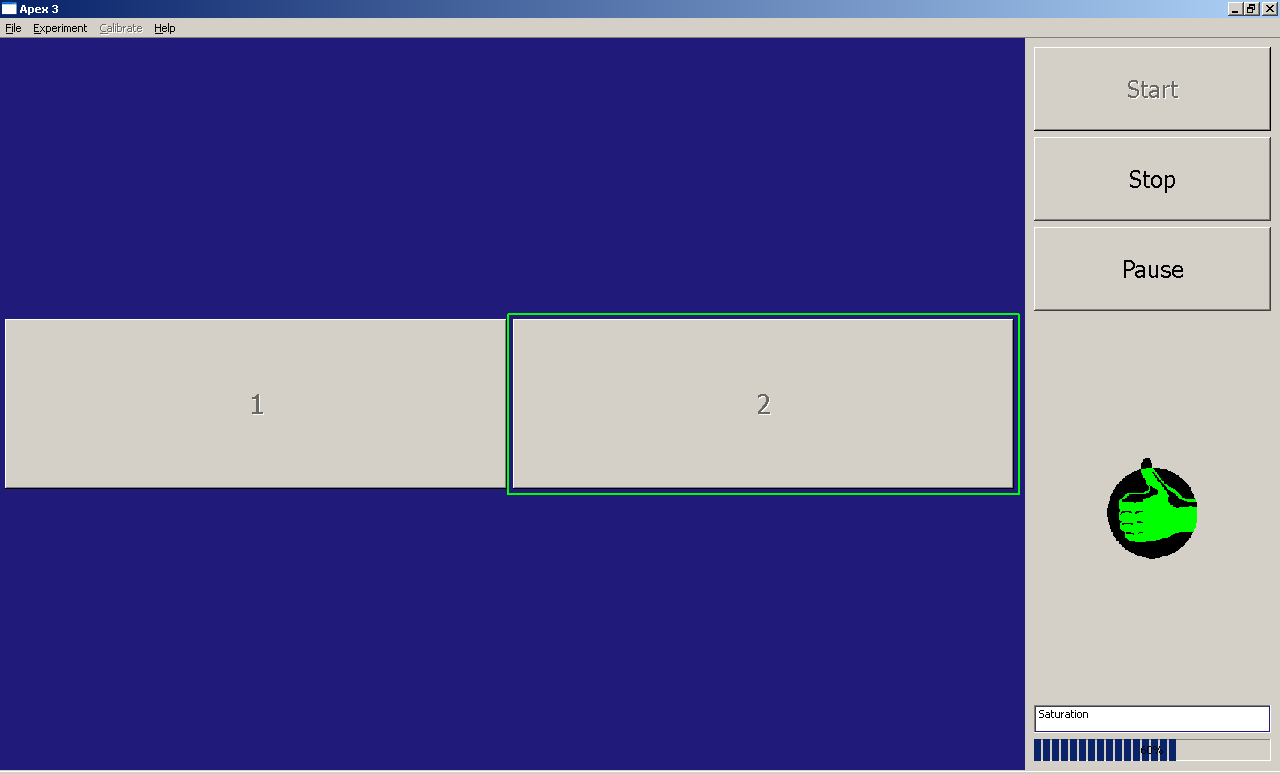
\includegraphics[width=\textwidth]{example3gapdetection.png}
 \caption{Example of adaptive gap detection experiment}
 \label{fig:gapdetection}
\end{figure}

\subsection{Conceptual}
The experiment as described in the previous paragraph should first
be translated to concepts understood by \apex. The main concepts
used here are \textbf{procedure}, \textbf{screens},
\textbf{datablocks} and \textbf{stimuli}.

For each wave file (noise with or without a gap) a \element
{datablocks} is defined, and for each datablock a \element
{stimulus} is defined. In this example there are 5 wave files,
with gap sizes ranging between 1 and 5 ms. Their IDs are
\id{g5ms}, \id{g4ms}, \id{g3ms},\id{g2ms} and \id{g1ms}. In an
adaptive procedure either a fixed or variable parameter is
defined. In this example a fixed parameter is used, i.e. the gap
size in the stimulus. The wave files with different gap sizes are
stored on disk, and are assigned a certain gap value. This gap
value is used to determine the gap threshold. Also, a \element
{screen} is defined that shows the two response intervals
indicating ``1'' and ``2''.

To indicate the order in which the stimuli should be presented a
\element {procedure} is defined. An adaptive procedure is defined
containing 1 \element {trial} with five variable stimuli (with
gap) and the standard stimulus without the gap. Recall that a
\element {trial} is the combination of a \element {screen} (always
the same in this example), a stimulus and a correct answer. The
standard and stimuli occur randomly in one of both intervals.

Now only the output logic remains to be defined. The idea is to
present the standard and a variable stimulus after each other, and
the stimulus to be presented depends on the response of the
subject. Filters are not used since the signals are not changed.

In the following sections each of the elements of the XML file
necessary to implement the latter concepts will be described in
detail.

\subsection{Detailed description of various elements}

\todo{modifications: to check, corrector?}
\begin{lstlisting} 
<procedure xsi:type="apex:adaptiveProcedure">
   <parameters>
     <presentations>1</presentations>
     <order>sequential</order>
     <intervals count="2">
	<interval number="1" element="button1"/>
	<interval number="2" element="button2"/>
	</intervals>
     <pause_between_stimuli>1000</pause_between_stimuli>
     <nUp>1</nUp>
     <nDown>2</nDown>
     <adapt_parameter>gap</adapt_parameter>
     <start_value>5</start_value>
     <stop_after_type>reversals</stop_after_type>
     <stop_after>5</stop_after>
     <min_value>0</min_value>
     <max_value>5</max_value>
     <larger_is_easier>true</larger_is_easier>
     <stepsizes>
       <change_after>reversals</change_after>
       <stepsize  begin="0" size="2"/>
       <stepsize begin="2" size="1"/>
     </stepsizes>
  </parameters>

  <trials>
    <trial id="trial1" >
     <screen id="screen1" />
     <stimulus id="stimulus1" />
     <stimulus id="stimulus2"/>
     <stimulus id="stimulus3"/>
     <stimulus id="stimulus4"/>
     <stimulus id="stimulus5"/>
     <standard id="standard"/>
    </trial>
  </trials>
</procedure>
\end{lstlisting}


\element{procedure} The attribute
\xml{xsi:type="adaptiveProcedureType"} refers to a procedure in which a parameter is changed according to
the response of the subject. In this example 1 trial is defined
with different stimuli from which the adaptive procedure chooses.

\begin{itemize}
\item \element{parameters} defines the behavior of the procedure
(eg., nr of presentations, order of presentation, response
strategy).

\begin{itemize}
\item \element{presentation} every trial is presented once.

\item \element{order} applies to the order of the trials. Since there is only 1
\element{trial}, it does not matter here wether the order is
specified as \element{sequential} or \element{random}.

\item \element{corrector} the corrector checks whether the
response is correct or not. In this example the number of choices
in \element{procedure} was 2. This means that \element{procedure}
will present the target stimulus in either interval 1 or 2.
\element{procedure} informs \element{corrector} about the correct
interval. \element{Corrector} also receives the clicked button from the
screen and looks up the corresponding number in the
\element{interval} element above and compares it with the number it
received from \element{procedure}. \todo{check}

\item \element{alternatives} number of alternatives to choose from
(here: 2 intervals) and the IDs of the buttons (defined under \element{screens} they correspond to.

\item \element{pause_between_stimuli} a pause of 1000 ms will be
introduced between successive wave files;

\item \element{nUp} number of items after incorrect trials to
increase the gap

\item \element{nDown} number of items after correct trials to
decrease the gap

\item \element{min_value} the gap size cannot be smaller than 0.

 \item \element{max_value} the gap size cannot be larger than 5

\item \element{adapt_parameter} the parameter to change, here the
``gap'', see also \element{fixed_parameters}

\item \element{start_value} the gap at which to start, here 5, see
under \element{stimulus}

\item \element{stop_after_type} reversals (it can also stop after
a number of presentations or trials)

\item \element{stop_after} number of reversals after which the
procedure is stopped

\item \element{rev_for_mean} the number of reversals that are used
for the average threshold

\item \element{larger_is_easier} here \xml{true} (the smaller the
gap, the more difficult the task)

\item \element{stepsizes} the stepsize

\end{itemize}

\begin{itemize}
\item\element{change_after} the \element{stepsize} is changed
after a specified number of reversals. In this example a stimulus
is skipped until the second reversal (start at 5, then 3, etc).
Thereafter no stimulus is skipped.

\end{itemize}

\item \element{trials} only 1 trial is defined

\begin{itemize}

\item \element{trial} the ID of the trial

\item\element{screen} the ID of the screen

\item \element{stimulus} the ID of the stimulus

\item \element{standard} the ID of the standard

\end{itemize}
\end{itemize}

\index{parameters}

\index{presentation}

\index{order}

\index{corrector}

\index{alternatives}

\index{pause between stimuli}

\index{nUp}

\index{nDown}

\index{adapt parameter}

\index{start value}

\index{stop after type}

\index{min value}

\index{max value}

\index{larger is easier}

\index{stepsize}

\index{trials}

\index{screen}

\index{stimulus}

\index{standard}



\begin{lstlisting}
<screens>
  <reinforcement>
    <progressbar>true</progressbar>
    <feedback length="300">true</feedback>
    <showcurrent>true</showcurrent>
  </reinforcement>

  <screen id="screen1" >
    <gridLayout height="1" width="2" id="main_layout">
      <button x="1" y="1" id="button1" >
       <text>1</text>
      </button>
      <button x="2" y="1" id="button2" >
       <text>2</text>
      </button>
    </gridLayout>
  <buttongroup id="buttongroup1">
     <button id="button1"/>
     <button id="button2"/>
  </buttongroup>
    <default_answer_element>buttongroup1</default_answer_element>
 </screen>
</screens>
\end{lstlisting}

\begin{itemize}
\item \element{screens} contains several screen elements that can
be referred to elsewhere in the experiment file (e.g. in
\element{procedure} above).


\item \element{reinforcement} includes elements on progress and
feedback

\begin{itemize}

\item \element{progressbar} if \xml {true} a progress bar will be
displayed in the right hand bottom corner of the screen. The
progress bar can indicate the percentage of trials that have been done or it
shows when a reversal occurs in an adaptive procedure. In the
latter case the progress bar will increase at every reversal while
the number of trials varies.

\item \element{feedback length} duration of the time after
response (in msec) that \apex waits before presenting the next
trial. During this interval feedback can be displayed.

\item \element{showcurrent} if \xml{true} the interval is highlighted while a
signal is presented.
\end{itemize}

\item \element{screen} each screen has an ID by which it can be
referred to elsewhere in the experiment. In this example the
screen displays two intervals.

\begin{itemize}


\item \element{gridlayout}places elements in an irregular grid.
The screen is divided into sections according to the values. In
this example there is an equal number of rows (x) and columns (y).

Gridlayout defines a group of screen elements (those that are
displayed on the screen).

\begin{itemize}
\item \element{button} for each interval a button is specified;
this button (interval) displays a number on the screen

\item \element{text} the left interval denotes ``1'', the right
one denotes ``2''.

\end{itemize}

\item \element{buttongroup} defines a group of screen elements
(those that are displayed on the screen). As many elements can be
defined in a screen, \apex has no way to know which element
contains the subject's response. Therefore, in
\element{default_answer_element} the element is designated that
contains the subject's response. In the case of screen elements
that are clicked in order to respond, the example is further
complicated by the fact that we cannot specify just one of the
elements (one button, one picture), but that the response rather comes
from a group of elements. This is when a \element{buttongroup} can
be used to group together different screen elements.

\end{itemize}
\end{itemize}



\index{screens}

\index{reinforcement}

\index{progressbar}

\index{feedback length}

\index{showcurrent}

\index{screen}

\index{gridlayout}

\index{button}

\index{text}

\index{buttongroup}

\index{default answer element}

\begin{lstlisting}
<datablocks>
  <uri_prefix>Gapfiles</uri_prefix>
    <datablock id="g5ms" >
      <device>wavdevice</device>
      <uri>g5.wav</uri>
    </datablock>

    <datablock id="g4ms" >
      <device>wavdevice</device>
      <uri>g4.wav</uri>
    </datablock>

    <datablock id="g3ms"  >
      <device>wavdevice</device>
      <uri>g3.wav</uri>
    </datablock>

    <datablock id="g2ms" >
      <device>wavdevice</device>
      <uri>g2.wav</uri>
    </datablock>

    <datablock id="g1ms"  >
      <device>wavdevice</device>
      <uri>g1.wav</uri>
    </datablock>

    <datablock id="datablockref">
      <device>wavdevice</device>
      <uri>ref500.wav</uri>
    </datablock>
  </datablocks>
\end{lstlisting}


\element{datablocks} contains a list of \element{datablock}
elements and a prefix.

\begin{itemize}
\item \element{uri_prefix}: a relative path is specified here.
Since \apex knows the location of the experiment file, only the
folder containing the wave files and pictures must be specified.



\item \element{datablock} for each wave file a unique datablock is
defined by an ID. The standard signal (uninterrupted noise) must
also be specified here.

\item \element{device} each datablock includes the audio device to
which the signal is routed

\item \element{uri} since the path is defined in
\element{uri_prefix} it is not necessary to specify the entire
path again

\index{datablocks} \index{uri prefix} \index{datablock}
\index{device} \index{uri}

\end{itemize}
\begin{lstlisting}
<devices>
 <device id="wavdevice" xsi:type="apex:wavDeviceType">
 <driver>portaudio</driver>
 <card>default</card>
 <channels>2</channels>
 <gain>0</gain>
 <samplerate>44100</samplerate>
 </device>
</devices>
\end{lstlisting}


\element{devices} all devices defined in the experiment file are
grouped in the \element{devices}. Only 1 \element{device} is used
in this example. The ID is set to soundcard. As an ID is unique
for an entire experiment file, it can be used later on to refer to
this device.

\begin{itemize}
\item \element{device} the \xml{xsi:type="apex:wavDeviceType"}
attribute tells \apex that a sound card is used. The experiment
only starts if all devices can be opened.

\item \element{driver} specifies the software driver to be used
for sound output. If unsure, set it to \xml{portaudio}.

\item \element{card} specifies the name of the sound card to be
used. The system default card can be used by specifying
\xml{default} as a card name. Other card names can be defined in
ApexConfig.

\item \element{channels} 2 channels are specified here, because
the signal is stereo.

\item \element{samplerate} the sampling frequency of the wave
files. Not all sampling rates are supported by all devices, and
some drivers automatically convert the sampling rate. Check your
sound card documentation. The sample rate of the sound card should
correspond to the sampling rates of all datablocks used with it.

\end{itemize}

\index{devices}

\index{driver}

\index{card}

\index{channels}

\index{gain}

\index{samplerate}


\begin{lstlisting}
<stimuli>
   <fixed_parameters>
     <parameter id="gap"/>
   </fixed_parameters>

   <stimulus id="stimulus1" >
     <description>noisewithgap1</description>
     <datablocks>
       <datablock id="g5ms" />
     </datablocks>
     <fixedParameters>
       <parameter id="gap">5</parameter>
     </fixedParameters>
   </stimulus>

   <stimulus id="stimulus2" >
     <description>noisewithgap2</description>
     <datablocks>
       <datablock id="g4ms" />
     </datablocks>
       <fixedParameters>
        <parameter id="gap">4</parameter>
     </fixedParameters>
   </stimulus>

   <stimulus id="stimulus3" >
     <description>noisewithgap3</description>
     <datablocks>
       <datablock id="g3ms" />
     </datablocks>
      <fixedParameters>
       <parameter id="gap">3</parameter>
      </fixedParameters>
   </stimulus>

   <stimulus id="stimulus4" >
     <description>noisewithgap4</description>
     <datablocks>
       <datablock id="g2ms" />
     </datablocks>
       <fixedParameters>
        <parameter id="gap">2</parameter>
       </fixedParameters>
   </stimulus>

   <stimulus id="stimulus5" >
     <description>noisewithgap5</description>
     <datablocks>
       <datablock id="g1ms" />
     </datablocks>
       <fixedParameters>
         <parameter id="gap">1</parameter>
       </fixedParameters>
   </stimulus>

   <stimulus id="standard">
     <datablocks>
      <datablock id="datablockref"/>
     </datablocks>
       <fixedParameters>
        <parameter id="gap">0</parameter>
     </fixedParameters>
   </stimulus>
</stimuli>
\end{lstlisting}


\element{stimuli} defines the auditory events, e.g. noise with gap
and noise without gap.

\begin{itemize}

\item \element{fixedParameters}

\begin{itemize}
\item \element{parameter} the gap is a fixed parameter that is
identified by an ID
\end{itemize}

\item \element{stimulus} this element includes a description of
the (variable) stimulus

\begin{itemize}
\item \element{description}

\item \element{datablocks} the ID refers to the wave file corresponding to the datablock

\item \element{fixedParameter}
\begin{itemize}
\item \element{parameter} includes information on the size of the
variable gap
\end{itemize}

\end{itemize}
\end{itemize}


\index{stimuli}

\index{fixed parameters}

\index{stimulus}

\index{datablocks}

\index{parameter}

\index{standard}

\begin{lstlisting}
<connections>
   <connection>
     <from>
       <id>_ALL_</id>
       <channel>0</channel>
     </from>
     <to>
       <id>wavdevice</id>
       <channel>1</channel>
     </to>
   </connection>

 </connections>
\end{lstlisting}

\index{connections} \index{channel}

\begin{itemize}
\item \element{connections} defines how the different datablocks
and filters are routed to the output device. The ID \id{_ALL_}
stands for all the datablocks. In this example they are routed to
1 channel of the wavdevice.
\end{itemize}

A visual representation of connections can be obtained by choosing
``Show stimulus connections'' under ``Experiment''in the main
\apex menu (top left menu bar).


\begin{lstlisting}
<results>
  <page>apex:resultsviewer.html</page>
  <resultparameters>
   <parameter name="reversals for mean">3</parameter>
  </resultparameters>
  <showduringexperiment>false</showduringexperiment>
  <showafterexperiment>true</showafterexperiment>
  <saveprocessedresults>true</saveprocessedresults>
 </results>
\end{lstlisting}

\element{results} Even if \element{results} is not specified in
the experiment file \apex will save a results file in XML. The results file
will display the correct answers, the reversals, the entire
sequence of responses, and the average threshold based on the
number of reversals and the magnitude of the corresponding gap
parameter specified in the experiment file.

\todo{new part, to check!}
\begin{itemize} 
\item \element{page} URL of the html page to show in the results window. The page should have the appropriate java script methods embedded. More example pages can be found in the \apex resultsviewer folder.
\item \element{resultparameters} Parameters to be passed to the results page. Each parameter will be set in hash params. \todo{perhaps some moren explanation on what this can be and why it is empty here?}
\item \element{showduringexperiment} If \xml{true}, an extra window will be created which will show the results of the current experiment while the experiment is being executed. Javascript embedded in the page will be executed upon each new trial.
\item \element{showafterexperiment} If \xml{true}, when the experiment is finished, a dialog box will appear querying whether results should be shown. If the answer is affirmative, a new window will be opened and the results will be shown after javascript processing.
\item \element{saveprocessedresults} If \xml{true} the
experimenter will be asked whether the processed results must be
appended to the results file. This will only work if the results are successfully saved to disk and your javascript code supports this transformation.
\end{itemize}

\index{results} \index{page} \index{resultparameters} \index{showduringexperiment} \index{showafterexperiment} \index{saveprocessedresults}



\begin{lstlisting}
 <general>
  <exitafter>true</exitafter>
 </general>
\end{lstlisting}

\element{general} defines some general parameters.

\begin{itemize}
\item \element{exitafter} if \xml{true} \apex will close after the experiment has ended and results have been shown.
\end{itemize}

\newpage
\section{Example 4: Gap detection in child mode}

\subsection{General description of the experiment}
See \filename{examples/manual/gapdetectionchild.apx}. This is an
example of a gap detection task adapted to the interest of
children: two stimuli are presented to the listener in random
order, a stationary noise and an interrupted noise. It is the same
experiment as example 3, but pictures (movies) of cars replace
buttons on the screen, and a smiley panel is
shown(figure~\ref{fig:gapchild}). During the presentation of
stimuli the cars are animated. The child's task is to indicate the
stimulus with the interruption. Feedback is provided by smileys
and the minimal detectable gap is determined by means of an
adaptive procedure (here 2-down, 1-up). Only those elements that
are specific to the child mode are described in this example.

\index{Example: gap detection - child mode}

\begin{figure}
 \centering
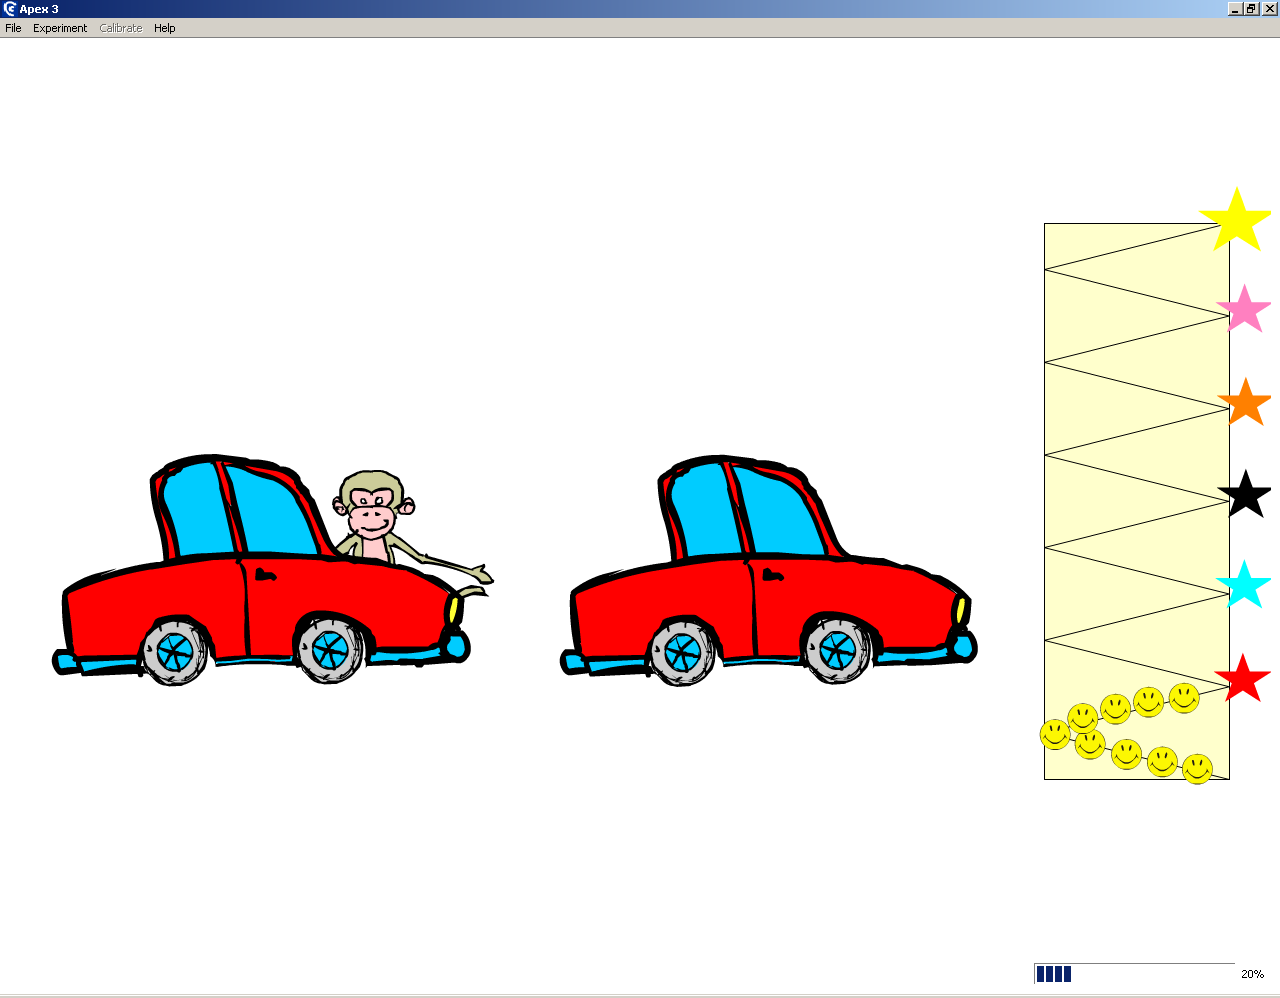
\includegraphics[width=\textwidth]{example4gapdetectionchild.png}
 \caption{Example of gap detection in child mode}
 \label{fig:gapchild}
\end{figure}

\subsection{Conceptual}
The main concepts illustrated in this example are
\textbf{childmode}, and \textbf{reinforcement}. Child mode
involves a different panel, and intro/outro movies.

\subsection{Detailed description of various elements}

\begin{lstlisting}
<screens>
    <uri_prefix>car/</uri_prefix>
    <general>
      <showpanel>true</showpanel>
    </general>
    <reinforcement>
      <progressbar>true</progressbar>
      <feedback length="300">true</feedback>
      <showcurrent>true</showcurrent>
    </reinforcement>
    <childmode>
      <panel>reinforcement.swf</panel>
    </childmode>
    <screen id="screen1">
      <gridLayout height="1" width="2" id="main_layout">
        <flash row="1" col="1" id="button1">
          <path>stillcar.swf</path>
          <feedback>
            <highlight>rijden.swf</highlight>
            <positive>goodcar.swf</positive>
            <negative>badcar.swf</negative>
          </feedback>
        </flash>

        <flash row="1" col="2" id="button2">
          <path>stillcar.swf</path>
          <feedback>
            <highlight>rijden.swf</highlight>
            <positive>goodcar.swf</positive>
            <negative>badcar.swf</negative>
          </feedback>
        </flash>
      </gridLayout>

      <buttongroup id="buttongroup1">
        <button id="button1"/>
        <button id="button2"/>
      </buttongroup>
      <default_answer_element>buttongroup1</default_answer_element>
    </screen>
  </screens>
\end{lstlisting}

\element{screens}

\begin{itemize}
\item \element{uri_prefix} a relative path is specified here
(relative with respect to the experiment file). This only applies
to the movies in \element{screen}. There are 3 ways to specify a
prefix: by directly specifying an absolute path, by directly
specifying a path relative to the experiment file or by referring
to a prefix stored in \filename{apexconfig.xml}. Please refer to
section~\ref{sec:prefixes} for more information.

\item \element{general}

\begin{itemize}

\item \element{show panel} if \xml {true} a panel will be shown
with smileys (see figure \textbf{presented above})

\end{itemize}

\item \element{reinforcement}
\begin{itemize}
\item \element{progressbar} If \xml {true} a progress bar will be
displayed on the right hand side with smileys. The progress bar
shows when a reversal occurs in an adaptive procedure (while the
number of trials varies).

\item \element{feedback length} duration of the time after
response (in msec) that \apex waits before presenting the next
trial. During this interval feedback can be displayed

\item \element{showcurrent} the interval is highlighted while a
signal is presented

\end{itemize}

\item\element{childmode} replaces the ``standard'' panel, sets
some defaults, enables intro/outro movies and changes the
background colour

\begin{itemize}

\item \element{panel} the name of the movie file, per frame
(smileys and panel are a collection of frames)

\end{itemize}

\end{itemize}

\element{screen} Each screen has an ID by which it can be referred
to elsewhere in the experiment. In this example the screen
displays two movies, each containing a car.

\begin{itemize}
\item \element{gridlayout} places elements in an irregular grid.
The screen is divided into sections according to the values. In
this example there are equal number of rows and columns.

\begin{itemize}
\item \element{flash} replaces \element{button} of the standard
version

\begin{itemize}
\item \element{path} the name of the flash movie file on disk,
when there is no animation.

\item \element{feedback}


\item \element{highlight}the name of the file while the car moves

\item \element{positive} the name of the movie file following a
correct response (here a monkey waving)

\item \element{negative} the name of the movie file following an
incorrect response  (the trunk of an elephant)

\end{itemize}

\end{itemize}

\item \element{buttongroup} defines a group of screen elements
(those that are displayed on the screen). As many elements can be
defined in a screen, \apex has no way to know which element
contains the subject's response. Therefore, in
\element{default_answer_element} the element is designated that
contains the subject's response. In the case of screen elements
that are clicked in order to respond, the example is further
complicated by the fact that we cannot specify just one of the
elements (buttons, pictures), but that the response rather comes
from a group of elements. This is when a \element{buttongroup} can
be used to group together different screen elements.


\end{itemize}
\index{screens}

\index{uri prefix}

\index{general}

\index{show panel}

\index{reinforcement}

\index{progressbar}

\index{feedback length}

\index{showcurrent}

\index{childmode}

\index{panel}

\index{screen}

\index{gridlayout}

\index{flash row}

\index{path}

\index{feedback}

\index{highlight}

\index{positive}

\index{negative}

\index{button}

\index{buttongroup}

\index{default answer element}

